% !TeX root = RJwrapper.tex
\title{mmpf: Monte-Carlo Methods for Prediction Functions}
\author{by Zachary M. Jones}

\maketitle

\abstract{
Machine learning methods can often learn high-dimensional functions which generalize well but are not human interpretable. \code{mmpf} marginalizes prediction functions using Monte-Carlo methods, allowing users to investigate the behavior of these learned functions as on a lower dimensional subset of input features: partial dependence and variations thereof. This makes machine learning methods more useful in situations where accurate prediction is not the only goal, such as in the social sciences where linear models are commonly used because of their interpretability.
}

Many methods for estimating prediction functions produce estimated functions which are not directly human-interpretable because of their complexity: they may include high-dimensional interactions and/or complex nonlinearities. While a learning method's capacity to automatically learn interactions and nonlinearities is attractive when the goal is prediction, there are many cases where users want good predictions \textit{and} the ability to understand how predictions depend on the features. \code{mmpf} implements general methods for interpreting prediction functions using Monte-Carlo methods. These methods allow any function which generates predictions to be be interpreted. \code{mmpf} is currently used in other packages for machine learning like \code{edarf} and \code{mlr} \citep{jones2016,JMLR:v17:15-066}.

\section{Marginalizing Prediction Functions}

The core function of \code{mmpf}, \code{marginalPrediction}, allows marginalization of a prediction function so that it depends on a subset of the features. Say the matrix of features $\mathbf{X}$ is partitioned into two subsets, $\mathbf{X}_u$ and $\mathbf{X}_{-u}$, where the former is of primary interest. A prediction function $f$ which in the regression case maps $\mathbf{X} \rightarrow \mathbf{y}$, where $\mathbf{y}$ is a real-valued vector might not be additive or linear in the columns of $\mathbf{X}_u$, making $f$ difficult to interpret directly. To obtain the marginal relationship between $\mathbf{X}_u$ and $f$ we could marginalize the joint distribution so that we obtain a function $f_u$ which only depends on the relevant subset of the features.

$$f_u (\mathbf{X}_u) = \int f(\mathbf{X}_u, \mathbf{X}_{-u}) \mathbb{P}(\mathbf{X}_u | \mathbf{X}_{-u}) \mathbb{P}(\mathbf{X}_{-u}) d \mathbf{X_{-u}} \label{eq:joint}$$

This however, can distort the relationship between $\mathbf{X}_u$ and $f$ because of the inclusion of dependence between $\mathbf{X}_u$ and $\mathbf{X}_{-u}$ (specifically $\mathbf{X}_u | \mathbf{X}_{-u}$), which is unrelated to $f$. An alternative is to instead integrate against the marginal distribution of $\mathbf{X}_{-u}$ as in \ref{eq:marginal}, as suggested by \citep{friedman2001greedy}.

$$\tilde{f}_u (\mathbf{X}_u) = \int f(\mathbf{X}_u, \mathbf{X}_{-u}) \mathbb{P}(\mathbf{X}_{-u}) d \mathbf{X_{-u}}  \label{eq:marginal}$$

\begin{figure}[h!]
  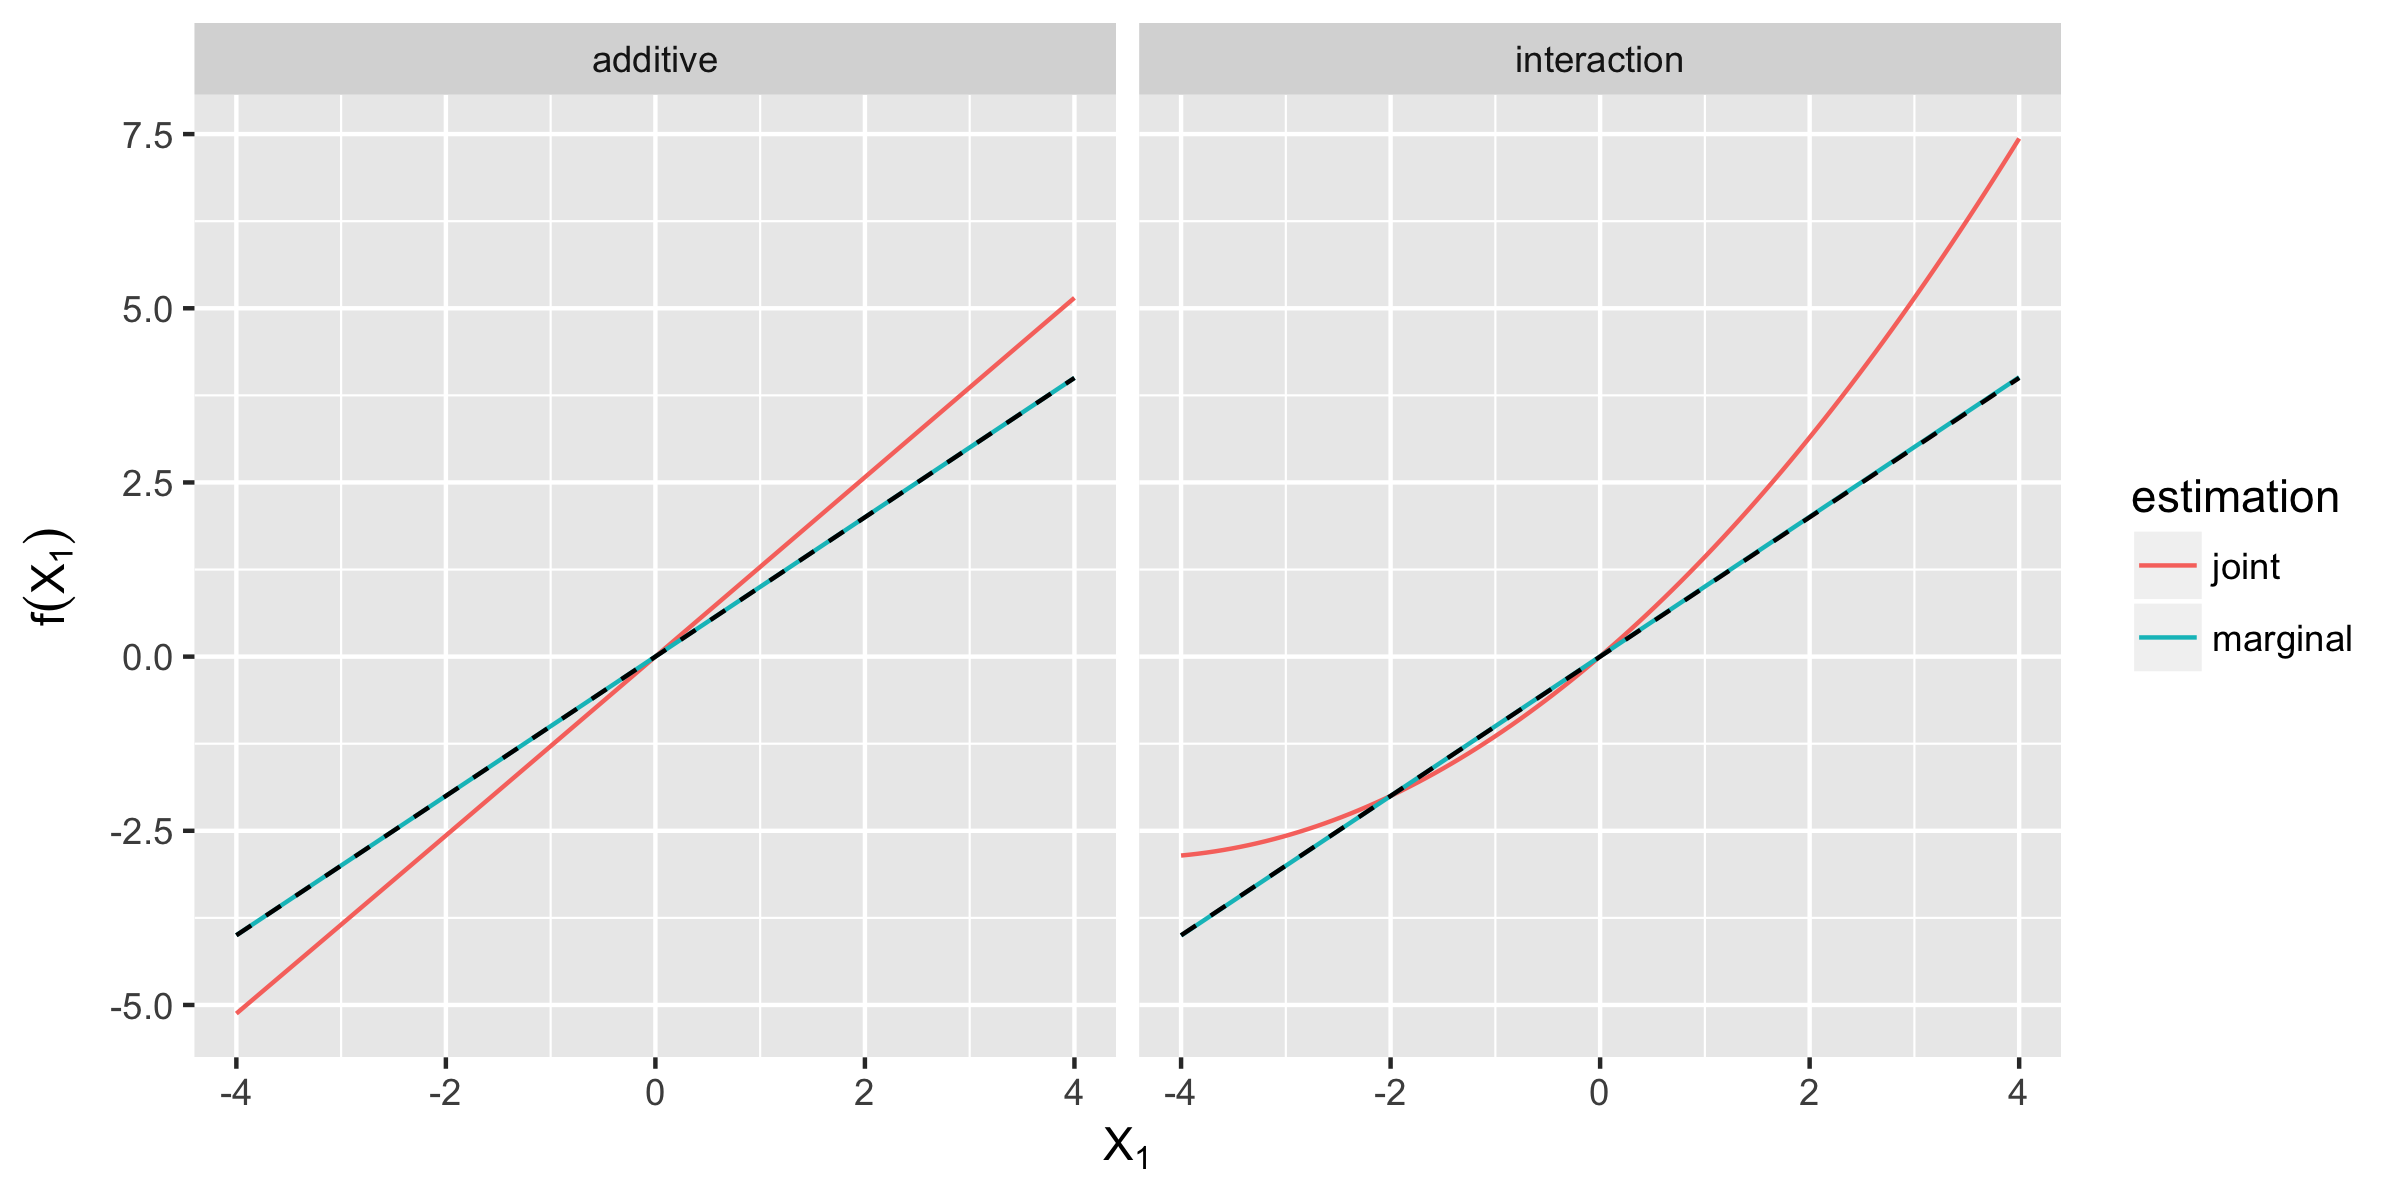
\includegraphics[width=\textwidth]{mvj.png}
  \caption{The marginal relationship between $\mathbf{x}_1$ and $f$ as estimated by integrating against the marginal distribution of $\mathbf{x}_2$ (the blue line) or the joint distribution of $(\mathbf{x}_1, \mathbf{x}_2)$ (the red line). The true relationship is shown by the dashed line. In the left panel $f$ is an additive function of $\mathbf{x}_1$ and $\mathbf{x}_2$ and in the right panel $\mathbf{x}_1$ and $\mathbf{x}_2$ interact via multiplication to produce $f$. \label{fig:sim}}
\end{figure}

To illustrate this point, suppose data are generated from an additive model, $f(\cdot) = \mathbf{\mathbf{x}_1} + \mathbf{\mathbf{x}_2}$ and $(\mathbf{x}_1, \mathbf{x}_2) \sim \text{MVN}(\mathbf{0}, \Sigma)$ where the diagonal entries of $\Sigma$ are $1$ and the off-diagonals are $.5$. That is, $(\mathbf{x}_1, \mathbf{x}_2)$ are correlated by construction. Now if we want to understand how $f$ depends on $\mathbf{x}_1$ we could integrate against the true joint distribution as in \ref{eq:joint}. However, this distorts the relationship between $\mathbf{x}_1$ and $f$ because the conditional probability of $\mathbf{x}_1$ given $\mathbf{x}_2$ is higher at values of $(\mathbf{x}_1, \mathbf{x}_2)$ which are more extreme (due to their correlation). Since $\mathbf{x}_2$ is related to $f$ this has the effect of distorting the relationship between $\mathbf{x}_1$ and $f$, and, in this case, makes the relationship appear more extreme than it is, as can be seen in the left panel of Figure \ref{fig:sim}. This distortion of the relationship between $\mathbf{x}_1$ and $f$ can be made more misleading if $\mathbf{x}_2$ interacts with $\mathbf{x}_1$ to produce $f$, or if $\mathbf{x}_2$ has a nonlinear relationship with $f$, as can be seen in the right panel of Figure \ref{fig:sim}.

Integrating against the marginal distribution of $\mathbf{x}_1$ recovers the true additive effect (left panel) and the average marginal effect ($\mathbf{x}_1 + .5 \mathbf{x}_1 \bar{\mathbf{x}_2}$, in the right panel) respectively.

\section{Using \code{mmpf}}

In practical settings we do not know $\mathbb{P}(\mathbf{X})$ or $f$. We can use $\hat{f}$, estimated from $(\mathbf{X}, \mathbf{y})$ as a plug-in estimator for $f$ and can estimate $\mathbb{P}(\mathbf{X}_{-u})$ from the training data, allowing us to estimate the \emph{partial dependence} of $\mathbf{X}_u$ on $\hat{f}$ \cite{friedman2001greedy}.

$$\hat{f}_u (\mathbf{X}_u) = \sum_{i = 1}^N \hat{f} (\mathbf{X}_u, \mathbf{X}_{-u}^{(i)}) \label{eq:pd}$$

This the behavior of the prediction function at a vector or matrix of values for $\mathbf{X}_u$, averaged over the empirical marginal distribution of $\mathbf{X}_{-u}$.

The core function of \code{mmpf}, \code{marginalPrediction}, allows users to compute partial dependence and many variations thereof easily. The key arguments of \code{marginalPrediction} are the prediction function (\code{predict.fun}), the training data (\code{data}), the names of the columns of the training data which are of interest (\code{vars}), the number of points to use in the grid for $\mathbf{X}_u$ and the number of points to sample from $\mathbf{X}_{-u}$ (\code{n}, an integer vector of length 2). Additional arguments control how the grid is constructed (e.g., uniform sampling, user chosen values, non-uniform sampling), allow the use of weights, and how aggregation is done (e.g., deviations from partial dependence). Below is an example using the Iris data \citep{anderson1936species}.

\begin{example}
  library(mmpf)
  library(randomForest)
  
  data(iris)
  iris.features = iris[, -ncol(iris)] # exclude the species column
  fit = randomForest(iris.features, iris$Species)

  mp = marginalPrediction(data = iris.features,
    vars = "Petal.Width",
    n = c(10, nrow(iris)), model = fit, uniform = TRUE,
    predict.fun = function(object, newdata) predict(object, newdata, type = "prob"))
  print(mp)
  ##     Petal.Width    setosa versicolor virginica
  ##  1:   0.1000000 0.6374133  0.2337733 0.1288133
  ##  2:   0.3666667 0.6374133  0.2337733 0.1288133
  ##  3:   0.6333333 0.6356267  0.2350533 0.1293200
  ##  4:   0.9000000 0.1707200  0.5997333 0.2295467
  ##  5:   1.1666667 0.1688267  0.6016267 0.2295467
  ##  6:   1.4333333 0.1688133  0.5880800 0.2431067
  ##  7:   1.7000000 0.1640400  0.4242800 0.4116800
  ##  8:   1.9666667 0.1619867  0.2066667 0.6313467
  ##  9:   2.2333333 0.1619867  0.2047867 0.6332267
  ## 10:   2.5000000 0.1619867  0.2047867 0.6332267
\end{example}

In this case $\hat{f}$ returns a probability of membership in each class for each values of the variable ``Petal.Width'' which is computed based on the average prediction for each value of ``Petal.Width'' shown and all the observed values of the other variables in the training data. As can be readily observed, partial dependence can be easily visualized, as in Figure \ref{figure:mp}.

\begin{figure}
  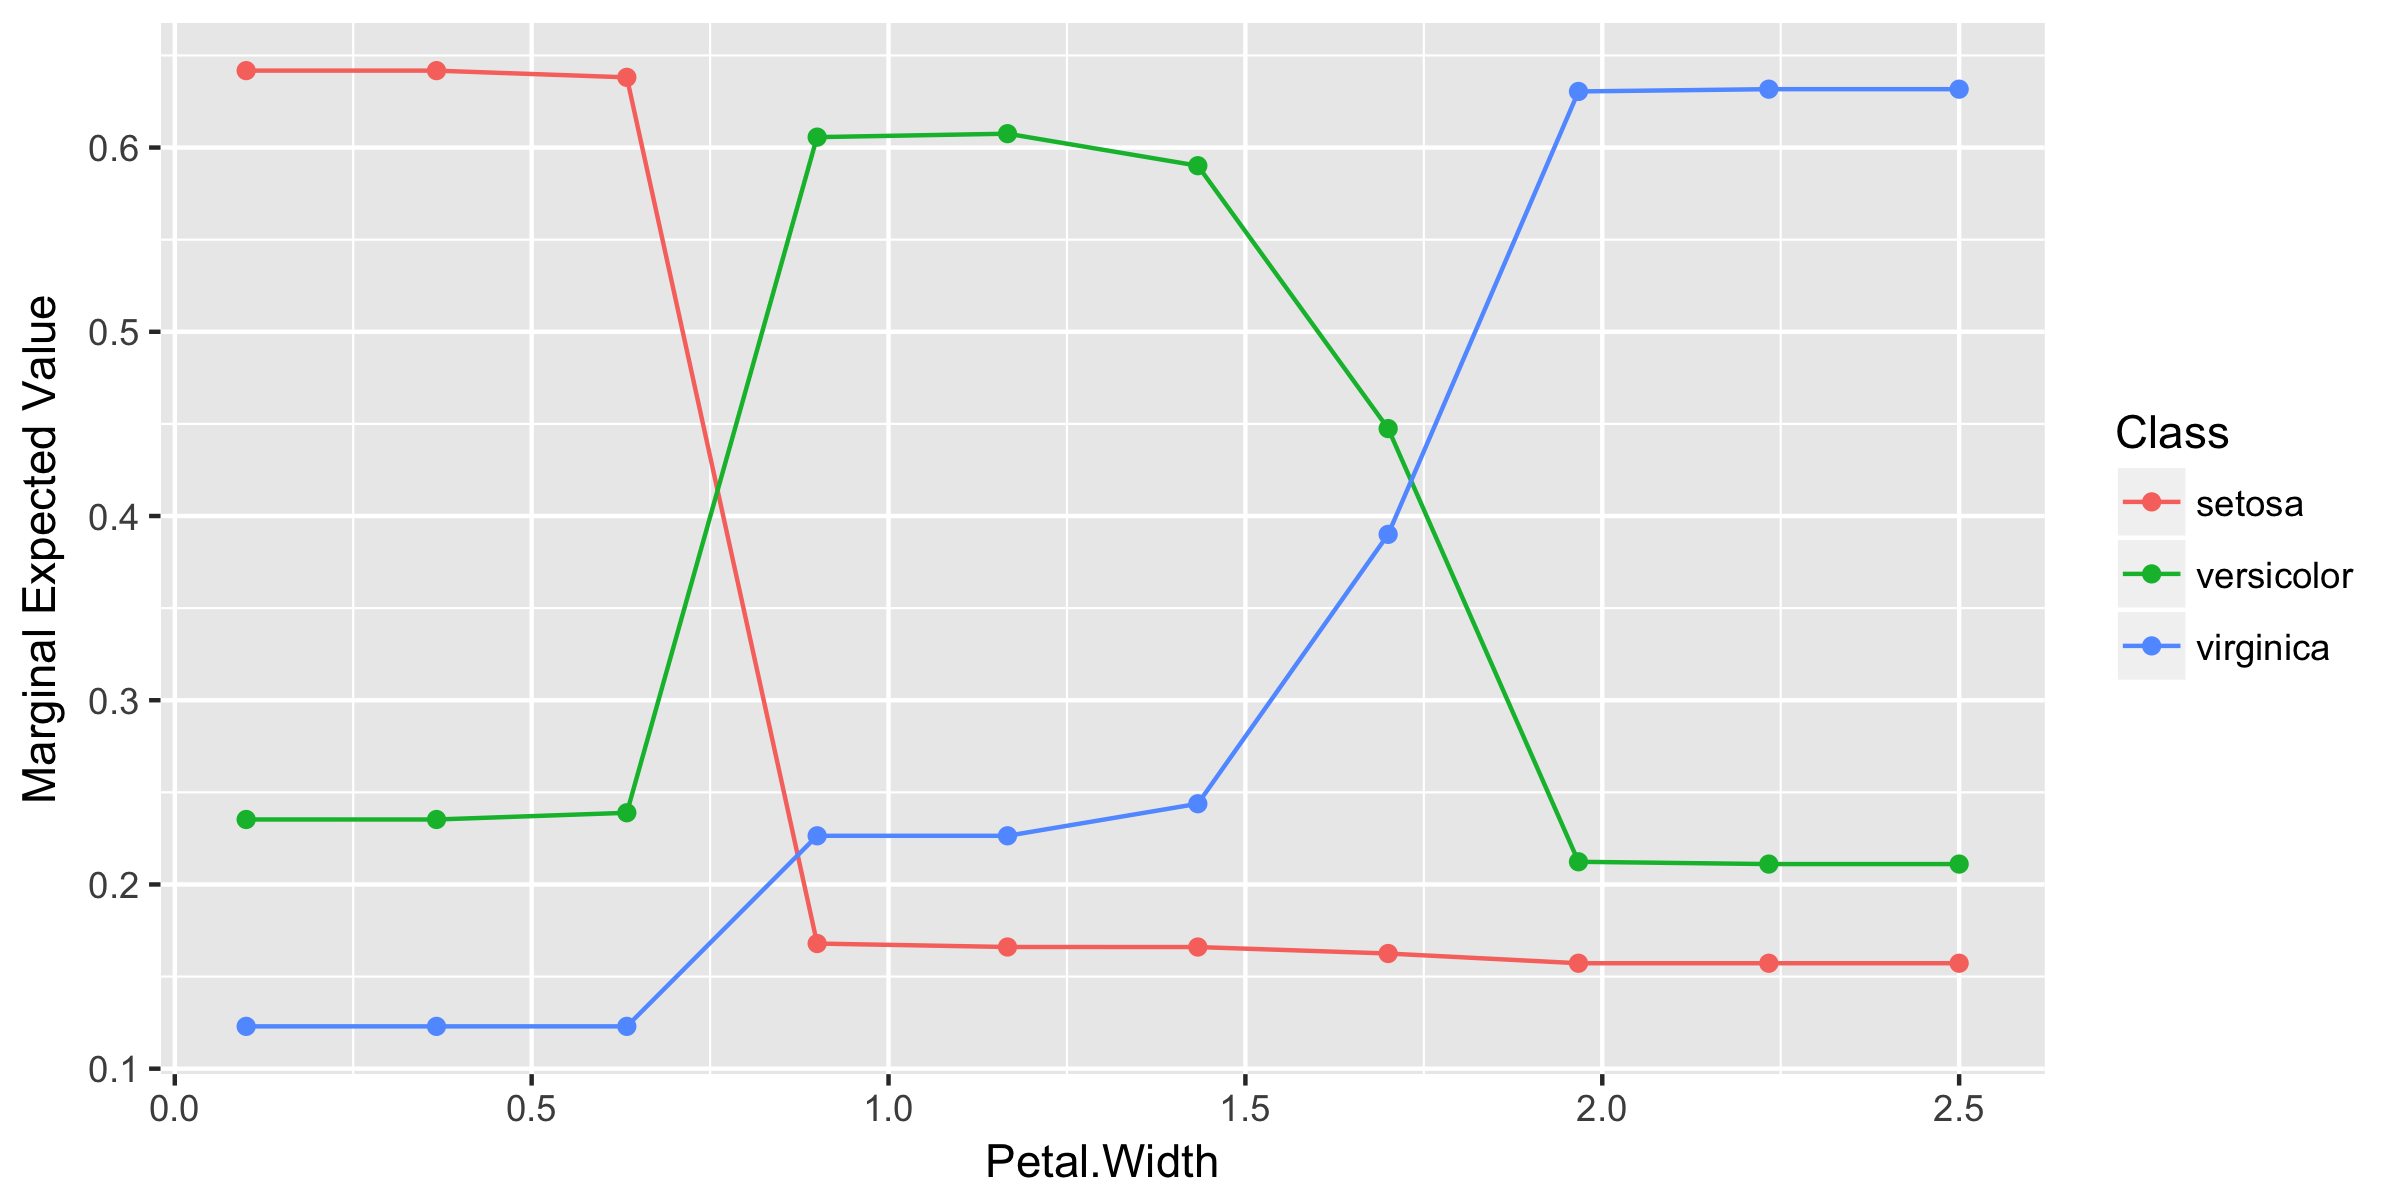
\includegraphics[width=\textwidth]{mp.png}
  \caption{The expected value of $\hat{f}$ estimated by a random forest and marginalized by Monte-Carlo integration to depend only on ``Petal.Width.'' \label{figure:mp}}
\end{figure}

In fact, \textit{any} function of the marginalized function $\hat{f}_u$ can be computed, including vector-valued functions. For example the expectation and variance of $\hat{f}_u$ can be simultaneously computed, the results of which are shown in Figures \ref{figure:mp_int_mean} and \ref{figure:mp_int_var}. Computing the variance of $\hat{f}_u$ can be used for detecting interactions between $\mathbf{X}_u$ and $\mathbf{X}_{-u}$ \citep{goldstein2015peeking}. If the variance of $\hat{f}_u(\mathbf{X}_u)$ is constant then this indicates that $\mathbf{X}_{-u}$ does not interact with $\mathbf{X}_u$, since, if it did, this would make $\hat{f}$ more variable in regions of the joint distribution wherein there is interaction between $\mathbf{X}_u$ and $\mathbf{X}_{-u}$.

\begin{example}
mp.int = marginalPrediction(data = iris.features,
  vars = c("Petal.Width", "Petal.Length"),
  n = c(10, nrow(iris)), model = fit, uniform = TRUE,
  predict.fun = function(object, newdata) predict(object, newdata, type = "prob"),
  aggregate.fun = function(x) list("mean" = mean(x), "variance" = var(x)))

head(mp.int)
##    Petal.Width Petal.Length setosa.mean setosa.variance versicolor.mean
## 1:         0.1     1.000000   0.9549867    0.0011619193      0.04448000
## 2:         0.1     1.655556   0.9549867    0.0011619193      0.04448000
## 3:         0.1     2.311111   0.9530933    0.0011317899      0.04637333
## 4:         0.1     2.966667   0.4574667    0.0003524653      0.52818667
## 5:         0.1     3.622222   0.4550400    0.0002619447      0.53061333
## 6:         0.1     4.277778   0.4550400    0.0002619447      0.52472000
##    versicolor.variance virginica.mean virginica.variance
## 1:         0.001141889   0.0005333333      0.00000239821
## 2:         0.001141889   0.0005333333      0.00000239821
## 3:         0.001112236   0.0005333333      0.00000239821
## 4:         0.001154918   0.0143466667      0.00054076492
## 5:         0.001016158   0.0143466667      0.00054076492
## 6:         0.001556364   0.0202400000      0.00093196886  
\end{example}

\begin{figure}
  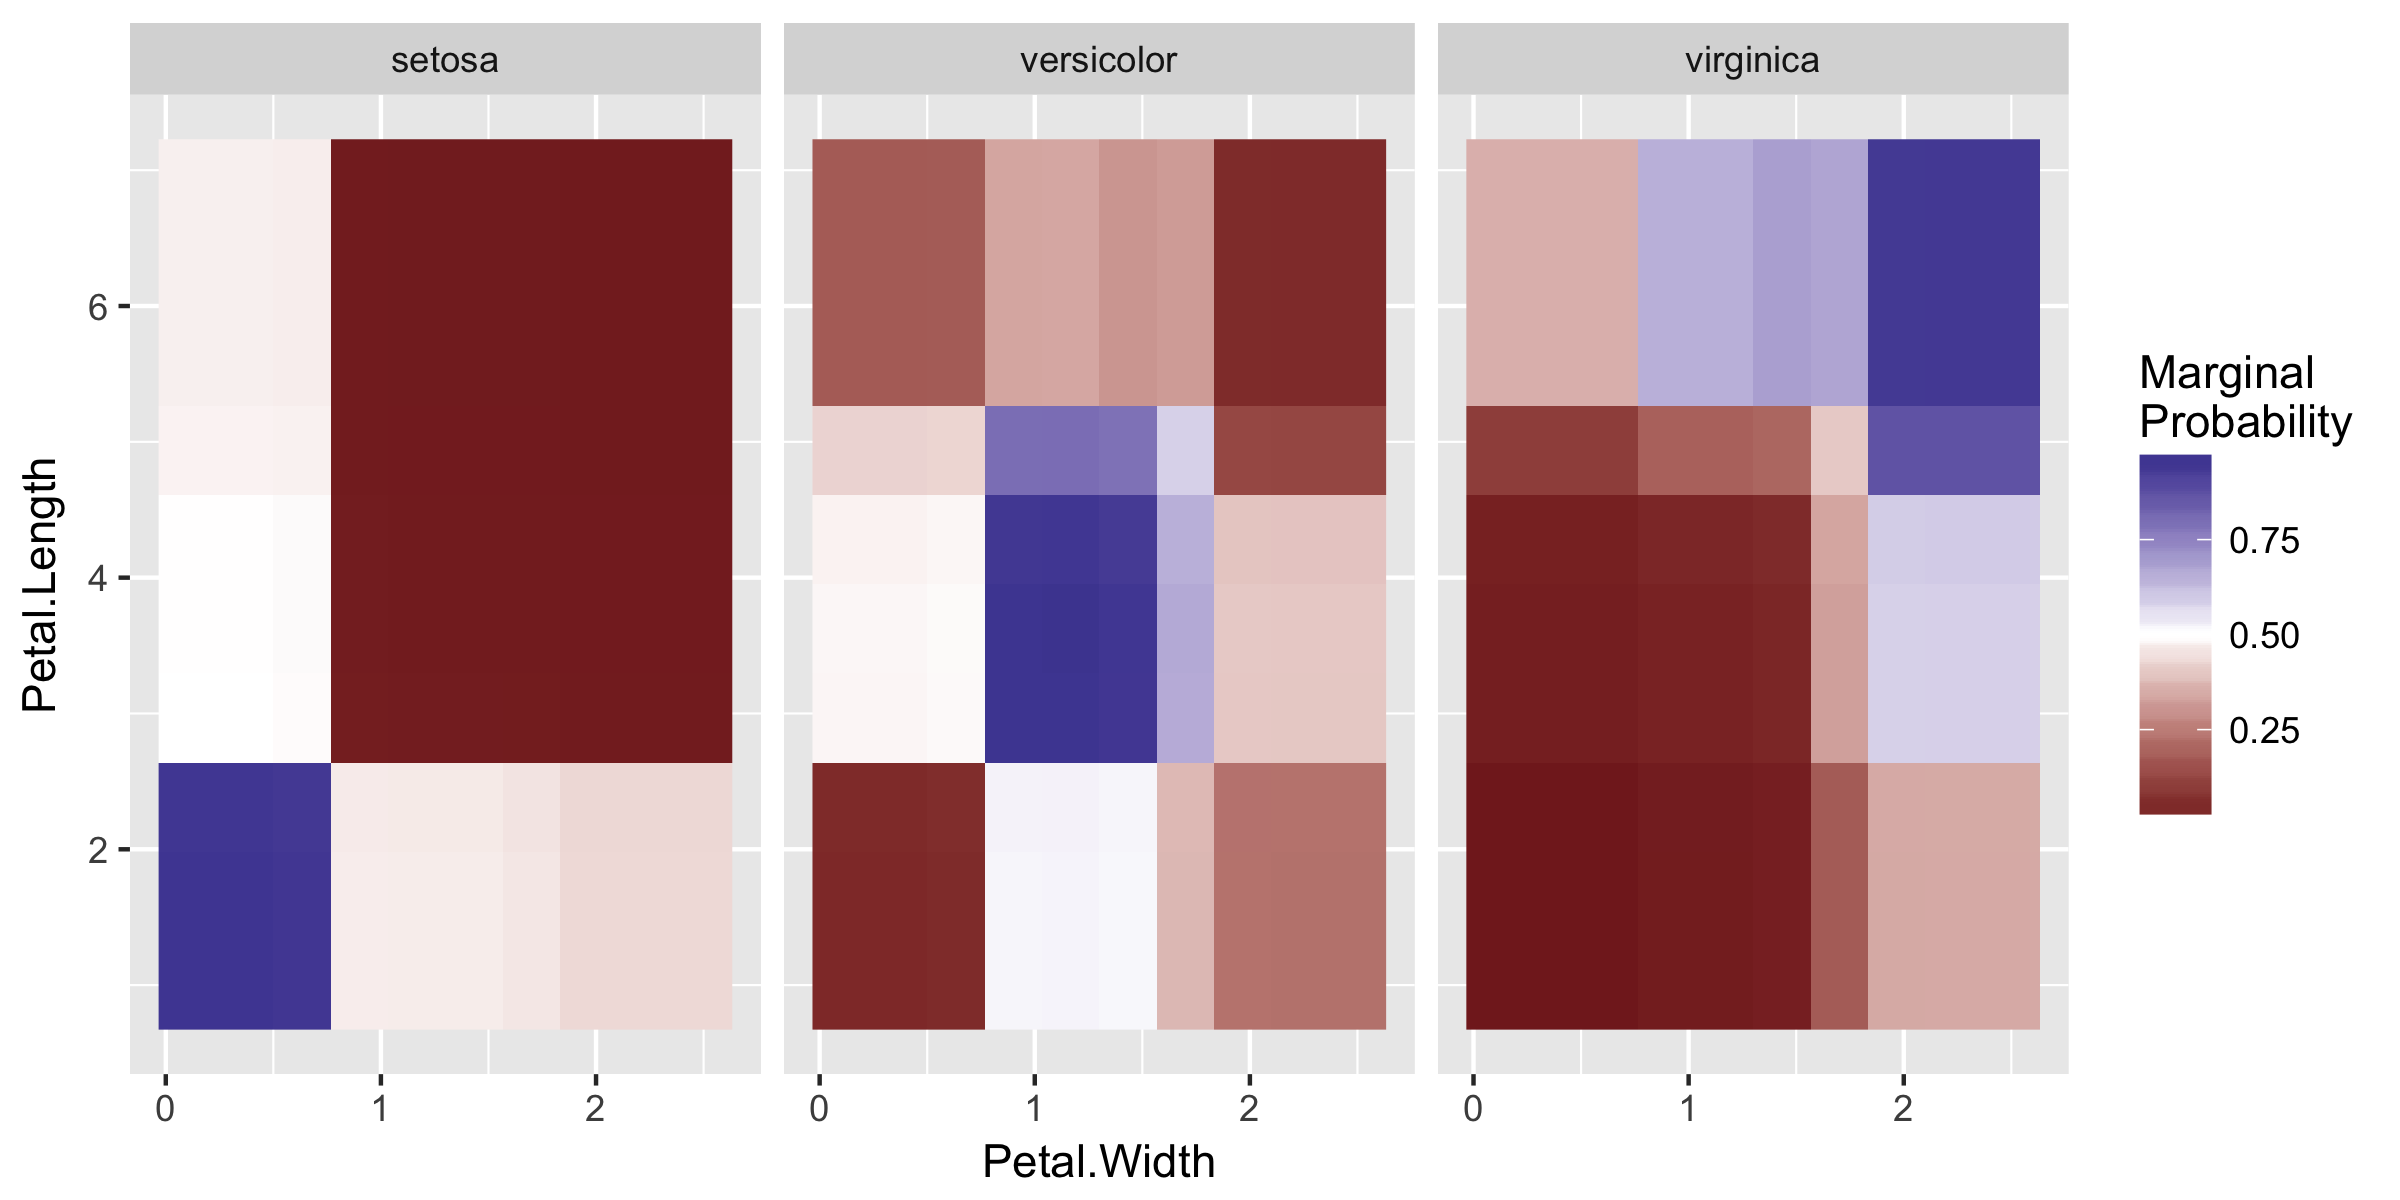
\includegraphics[width=\textwidth]{mp_int_mean.png}
  \caption{The expected value of $\hat{f}$ estimated by a random forest and marginalized by Monte-Carlo integration to depend only on ``Petal.Width'' and ``Petal.Length.'' \label{figure:mp_int_mean}}
\end{figure}

\begin{figure}
  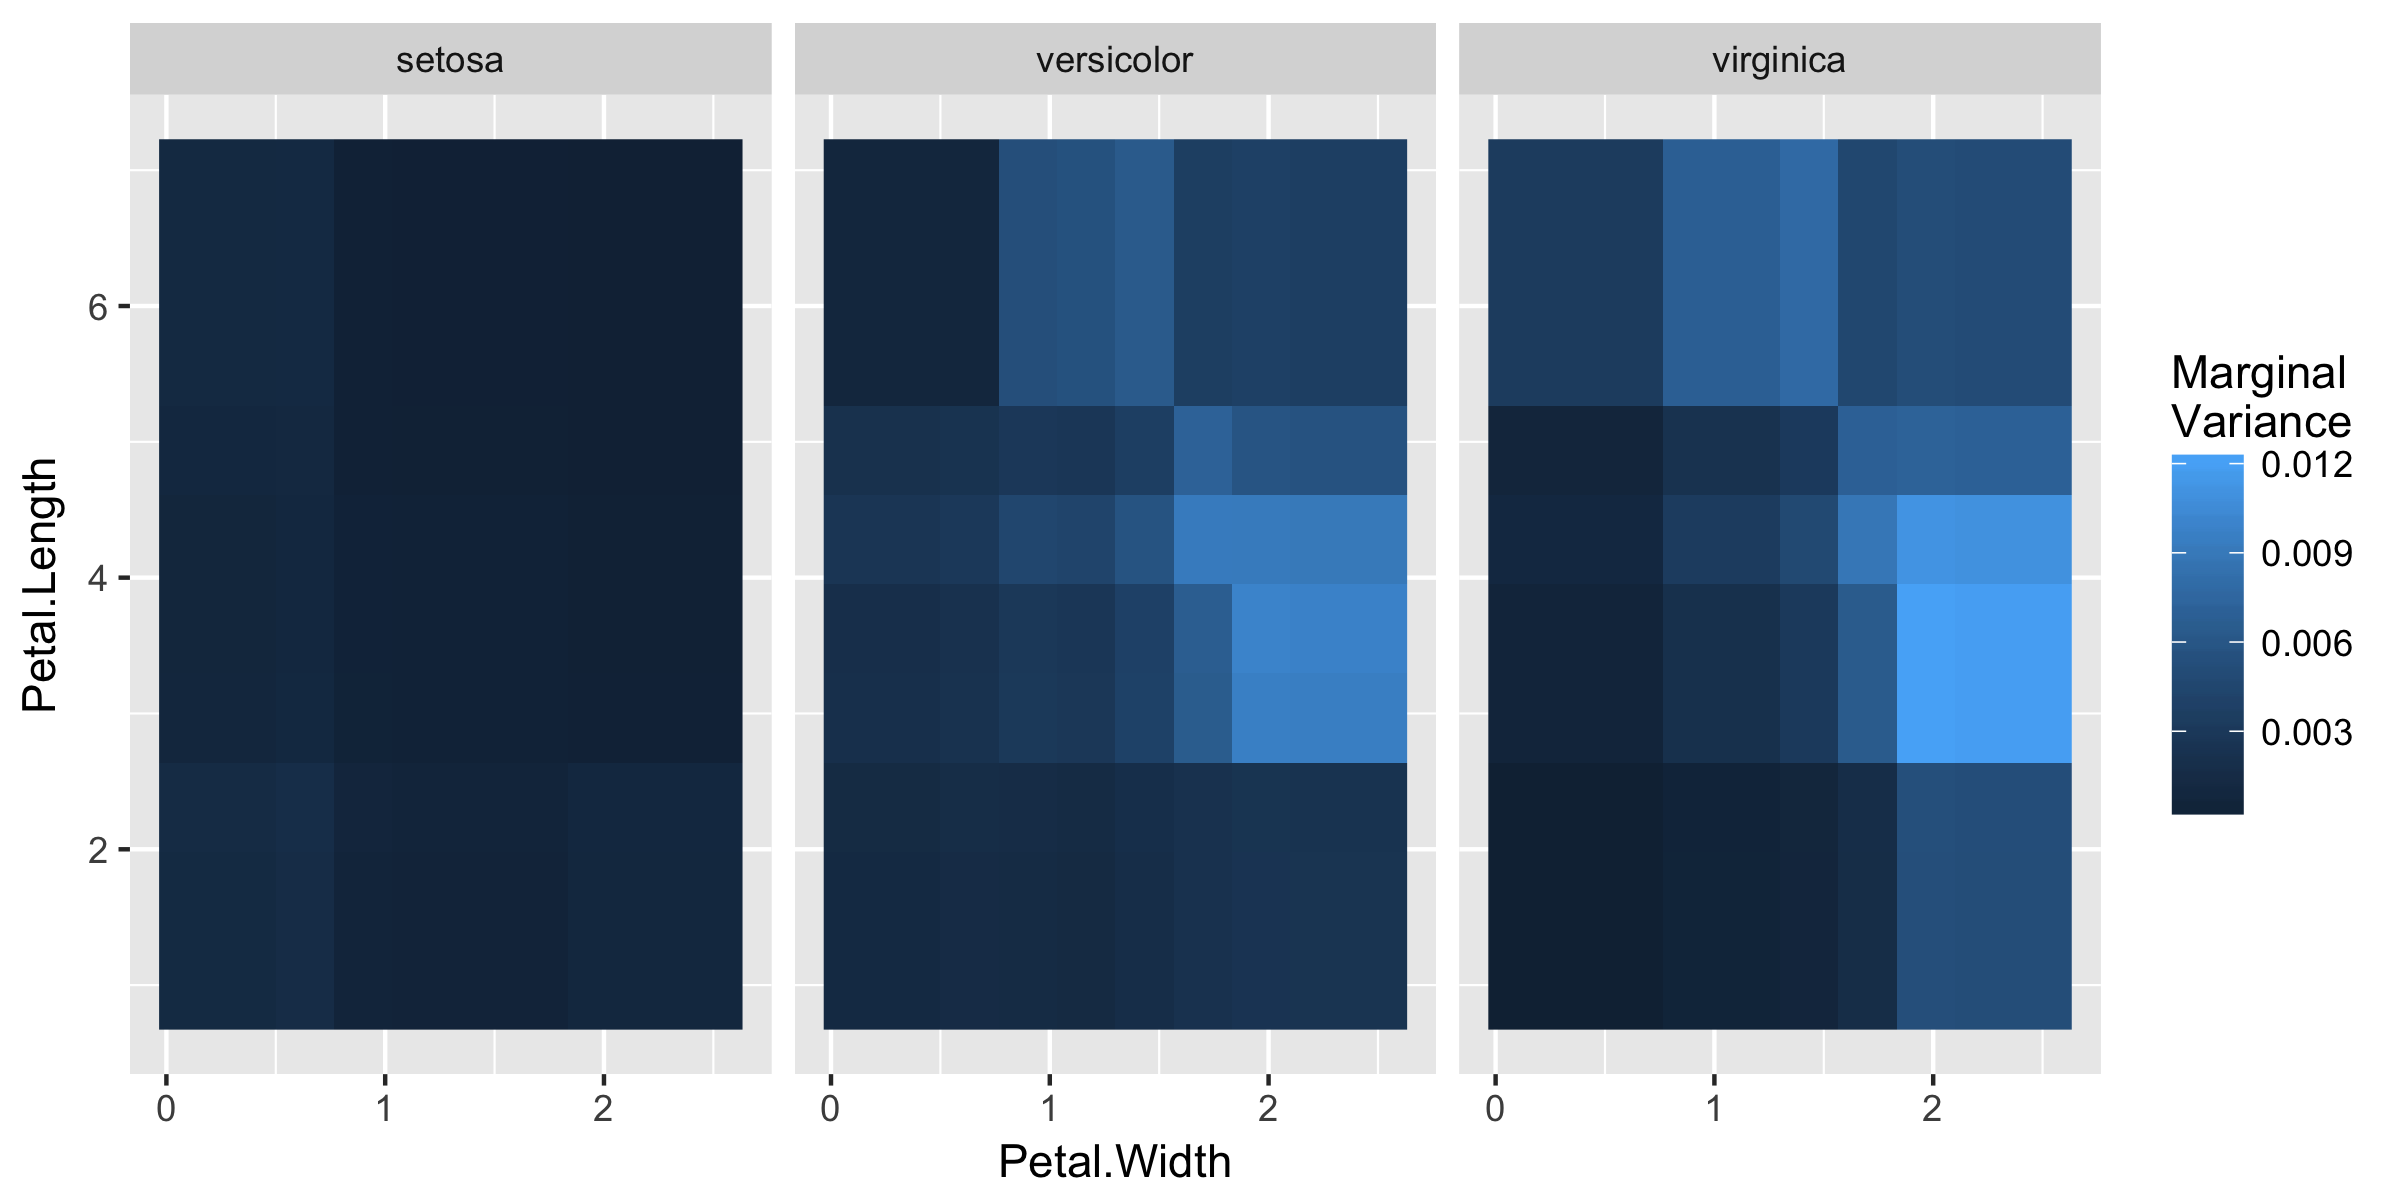
\includegraphics[width=\textwidth]{mp_int_var.png}
  \caption{The variance of $\hat{f}$ estimated by a random forest and marginalized by Monte-Carlo integration to depend only on ``Petal.Width'' and ``Petal.Length.'' Non-constant variance indicates interaction between these variables and those marginalized out of $\hat{f}$. \label{figure:mp_int_var}}
\end{figure}

\clearpage
\newpage

\bibliography{jones}

\address{Zachary M. Jones\\
  Pennsylvania State University\\
  University Park, Pennsylvania\\
  United States\\}
\email{zmj@zmjones.com}